% Options for packages loaded elsewhere
\PassOptionsToPackage{unicode}{hyperref}
\PassOptionsToPackage{hyphens}{url}
%
\documentclass[
]{article}
\usepackage{amsmath,amssymb}
\usepackage{lmodern}
\usepackage{ifxetex,ifluatex}
\ifnum 0\ifxetex 1\fi\ifluatex 1\fi=0 % if pdftex
  \usepackage[T1]{fontenc}
  \usepackage[utf8]{inputenc}
  \usepackage{textcomp} % provide euro and other symbols
\else % if luatex or xetex
  \usepackage{unicode-math}
  \defaultfontfeatures{Scale=MatchLowercase}
  \defaultfontfeatures[\rmfamily]{Ligatures=TeX,Scale=1}
\fi
% Use upquote if available, for straight quotes in verbatim environments
\IfFileExists{upquote.sty}{\usepackage{upquote}}{}
\IfFileExists{microtype.sty}{% use microtype if available
  \usepackage[]{microtype}
  \UseMicrotypeSet[protrusion]{basicmath} % disable protrusion for tt fonts
}{}
\makeatletter
\@ifundefined{KOMAClassName}{% if non-KOMA class
  \IfFileExists{parskip.sty}{%
    \usepackage{parskip}
  }{% else
    \setlength{\parindent}{0pt}
    \setlength{\parskip}{6pt plus 2pt minus 1pt}}
}{% if KOMA class
  \KOMAoptions{parskip=half}}
\makeatother
\usepackage{xcolor}
\IfFileExists{xurl.sty}{\usepackage{xurl}}{} % add URL line breaks if available
\IfFileExists{bookmark.sty}{\usepackage{bookmark}}{\usepackage{hyperref}}
\hypersetup{
  pdftitle={HW week 11},
  pdfauthor={Da Qi Ren},
  hidelinks,
  pdfcreator={LaTeX via pandoc}}
\urlstyle{same} % disable monospaced font for URLs
\usepackage[margin=1in]{geometry}
\usepackage{color}
\usepackage{fancyvrb}
\newcommand{\VerbBar}{|}
\newcommand{\VERB}{\Verb[commandchars=\\\{\}]}
\DefineVerbatimEnvironment{Highlighting}{Verbatim}{commandchars=\\\{\}}
% Add ',fontsize=\small' for more characters per line
\usepackage{framed}
\definecolor{shadecolor}{RGB}{248,248,248}
\newenvironment{Shaded}{\begin{snugshade}}{\end{snugshade}}
\newcommand{\AlertTok}[1]{\textcolor[rgb]{0.94,0.16,0.16}{#1}}
\newcommand{\AnnotationTok}[1]{\textcolor[rgb]{0.56,0.35,0.01}{\textbf{\textit{#1}}}}
\newcommand{\AttributeTok}[1]{\textcolor[rgb]{0.77,0.63,0.00}{#1}}
\newcommand{\BaseNTok}[1]{\textcolor[rgb]{0.00,0.00,0.81}{#1}}
\newcommand{\BuiltInTok}[1]{#1}
\newcommand{\CharTok}[1]{\textcolor[rgb]{0.31,0.60,0.02}{#1}}
\newcommand{\CommentTok}[1]{\textcolor[rgb]{0.56,0.35,0.01}{\textit{#1}}}
\newcommand{\CommentVarTok}[1]{\textcolor[rgb]{0.56,0.35,0.01}{\textbf{\textit{#1}}}}
\newcommand{\ConstantTok}[1]{\textcolor[rgb]{0.00,0.00,0.00}{#1}}
\newcommand{\ControlFlowTok}[1]{\textcolor[rgb]{0.13,0.29,0.53}{\textbf{#1}}}
\newcommand{\DataTypeTok}[1]{\textcolor[rgb]{0.13,0.29,0.53}{#1}}
\newcommand{\DecValTok}[1]{\textcolor[rgb]{0.00,0.00,0.81}{#1}}
\newcommand{\DocumentationTok}[1]{\textcolor[rgb]{0.56,0.35,0.01}{\textbf{\textit{#1}}}}
\newcommand{\ErrorTok}[1]{\textcolor[rgb]{0.64,0.00,0.00}{\textbf{#1}}}
\newcommand{\ExtensionTok}[1]{#1}
\newcommand{\FloatTok}[1]{\textcolor[rgb]{0.00,0.00,0.81}{#1}}
\newcommand{\FunctionTok}[1]{\textcolor[rgb]{0.00,0.00,0.00}{#1}}
\newcommand{\ImportTok}[1]{#1}
\newcommand{\InformationTok}[1]{\textcolor[rgb]{0.56,0.35,0.01}{\textbf{\textit{#1}}}}
\newcommand{\KeywordTok}[1]{\textcolor[rgb]{0.13,0.29,0.53}{\textbf{#1}}}
\newcommand{\NormalTok}[1]{#1}
\newcommand{\OperatorTok}[1]{\textcolor[rgb]{0.81,0.36,0.00}{\textbf{#1}}}
\newcommand{\OtherTok}[1]{\textcolor[rgb]{0.56,0.35,0.01}{#1}}
\newcommand{\PreprocessorTok}[1]{\textcolor[rgb]{0.56,0.35,0.01}{\textit{#1}}}
\newcommand{\RegionMarkerTok}[1]{#1}
\newcommand{\SpecialCharTok}[1]{\textcolor[rgb]{0.00,0.00,0.00}{#1}}
\newcommand{\SpecialStringTok}[1]{\textcolor[rgb]{0.31,0.60,0.02}{#1}}
\newcommand{\StringTok}[1]{\textcolor[rgb]{0.31,0.60,0.02}{#1}}
\newcommand{\VariableTok}[1]{\textcolor[rgb]{0.00,0.00,0.00}{#1}}
\newcommand{\VerbatimStringTok}[1]{\textcolor[rgb]{0.31,0.60,0.02}{#1}}
\newcommand{\WarningTok}[1]{\textcolor[rgb]{0.56,0.35,0.01}{\textbf{\textit{#1}}}}
\usepackage{graphicx}
\makeatletter
\def\maxwidth{\ifdim\Gin@nat@width>\linewidth\linewidth\else\Gin@nat@width\fi}
\def\maxheight{\ifdim\Gin@nat@height>\textheight\textheight\else\Gin@nat@height\fi}
\makeatother
% Scale images if necessary, so that they will not overflow the page
% margins by default, and it is still possible to overwrite the defaults
% using explicit options in \includegraphics[width, height, ...]{}
\setkeys{Gin}{width=\maxwidth,height=\maxheight,keepaspectratio}
% Set default figure placement to htbp
\makeatletter
\def\fps@figure{htbp}
\makeatother
\setlength{\emergencystretch}{3em} % prevent overfull lines
\providecommand{\tightlist}{%
  \setlength{\itemsep}{0pt}\setlength{\parskip}{0pt}}
\setcounter{secnumdepth}{-\maxdimen} % remove section numbering
\usepackage{booktabs}
\usepackage{longtable}
\usepackage{array}
\usepackage{multirow}
\usepackage{wrapfig}
\usepackage{float}
\usepackage{colortbl}
\usepackage{pdflscape}
\usepackage{tabu}
\usepackage{threeparttable}
\usepackage{threeparttablex}
\usepackage[normalem]{ulem}
\usepackage{makecell}
\usepackage{xcolor}
\ifluatex
  \usepackage{selnolig}  % disable illegal ligatures
\fi

\title{HW week 11}
\usepackage{etoolbox}
\makeatletter
\providecommand{\subtitle}[1]{% add subtitle to \maketitle
  \apptocmd{\@title}{\par {\large #1 \par}}{}{}
}
\makeatother
\subtitle{w203: Statistics for Data Science}
\author{Da Qi Ren}
\date{}

\begin{document}
\maketitle

\newcommand{\E}{\text{E}}
\newcommand{\V}{\text{V}}
\newcommand{\R}{\mathbb{R}}
\newcommand{\Cov}{\mathbb{\text{Cov}}}

\hypertarget{regression-analysis-of-youtube-dataset}{%
\subsection{Regression analysis of YouTube
dataset}\label{regression-analysis-of-youtube-dataset}}

You want to explain how much the quality of a video affects the number
of views it receives on social media. \textbf{This is a causal
question.}

You will use a dataset created by Cheng, Dale and Liu at Simon Fraser
University. It includes observations about 9618 videos shared on
YouTube. Please see \href{http://netsg.cs.sfu.ca/youtubedata/}{this
link} for details about how the data was collected.

You will use the following variables:

\begin{itemize}
\item
  views: the number of views by YouTube users.
\item
  rate: the average rating given by users.
\item
  length: the duration of the video in seconds.
\end{itemize}

You want to use the \texttt{rate} variable as a proxy for video quality.
You also include \texttt{length} as a control variable. You estimate the
following ols regression:

\[\text{views} =   789 +  2103    \text{ rate} +      3.00 \text{ length} \]
a. Name an omitted variable that you think could induce significant
omitted variable bias. Argue whether the direction of bias is towards
zero or away from zero.

ANSWER:

I answer this question in 2 ways:

(Method 1) Name an omitted variable ``recommendation'' representing if
the video is recommended by the system, this data is not in the given
data set. Therefore,

\hypertarget{textviews-789-2103-text-rate-3.00-text-length-beta-times-recommendation}{%
\section{\texorpdfstring{\[\text{views} =   789 +  2103    \text{ rate} +      3.00 \text{ length} + \beta \times recommendation  \]}{\textbackslash text\{views\} =   789 +  2103    \textbackslash text\{ rate\} +      3.00 \textbackslash text\{ length\} + \textbackslash beta \textbackslash times recommendation  }}\label{textviews-789-2103-text-rate-3.00-text-length-beta-times-recommendation}}

\hypertarget{text-ate-alpha_0-alpha_1-times-recommendation}{%
\section{\texorpdfstring{\[\text{ ate} =\alpha_0 + \alpha_1 \times recommendation  \]}{\textbackslash text\{ ate\} =\textbackslash alpha\_0 + \textbackslash alpha\_1 \textbackslash times recommendation  }}\label{text-ate-alpha_0-alpha_1-times-recommendation}}

\hypertarget{if-beta2-0-and-alpha1-0-then-omvb-beta2-times-alpha1-0-.-and-if-beta1-0}{%
\section{\texorpdfstring{\[if\  \beta2 > 0\  and\    \alpha1 > 0 \  then\ OMVB =   \beta2 \times \alpha1 > 0 . \ And,  \  \  if \  \beta1 > 0 \]}{if\textbackslash{}  \textbackslash beta2 \textgreater{} 0\textbackslash{}  and\textbackslash{}    \textbackslash alpha1 \textgreater{} 0 \textbackslash{}  then\textbackslash{} OMVB =   \textbackslash beta2 \textbackslash times \textbackslash alpha1 \textgreater{} 0 . \textbackslash{} And,  \textbackslash{}  \textbackslash{}  if \textbackslash{}  \textbackslash beta1 \textgreater{} 0 }}\label{if-beta2-0-and-alpha1-0-then-omvb-beta2-times-alpha1-0-.-and-if-beta1-0}}

\hypertarget{the-ols-coefficient-on-views-will-scaled-away-from-zero-more-positive-gaining-statistical-significance.}{%
\section{the OLS coefficient on views will scaled away from zero (more
positive) gaining statistical
significance.}\label{the-ols-coefficient-on-views-will-scaled-away-from-zero-more-positive-gaining-statistical-significance.}}

\newpage

(Method 2) Using the data in videos.csv file. Estimator Positively
Biased Away from Zero In this case, we have an estimator that is biased
in the positive direction. Since the coefficient that it is associated
with is positive as well we would say it is biased away from zero. We
break down the components of the omitted variable bias below.

\begin{Shaded}
\begin{Highlighting}[]
\NormalTok{df}\OtherTok{\textless{}{-}}\FunctionTok{read.csv}\NormalTok{(}\StringTok{\textquotesingle{}videos001.csv\textquotesingle{}}\NormalTok{)}

\CommentTok{\#df\textless{}{-}df \%\textgreater{}\% }
\CommentTok{\#  select(\textquotesingle{}rate\textquotesingle{}, \textquotesingle{}views\textquotesingle{}, \textquotesingle{}length\textquotesingle{}, \textquotesingle{}ratings\textquotesingle{}) }
\NormalTok{df }\OtherTok{\textless{}{-}} \FunctionTok{subset}\NormalTok{(df, }\AttributeTok{select =} \FunctionTok{c}\NormalTok{(}\StringTok{\textquotesingle{}rate\textquotesingle{}}\NormalTok{, }\StringTok{\textquotesingle{}views\textquotesingle{}}\NormalTok{, }\StringTok{\textquotesingle{}length\textquotesingle{}}\NormalTok{, }\StringTok{\textquotesingle{}ratings\textquotesingle{}}\NormalTok{))  }
\FunctionTok{nrow}\NormalTok{(df)}
\end{Highlighting}
\end{Shaded}

\begin{verbatim}
## [1] 9617
\end{verbatim}

\begin{Shaded}
\begin{Highlighting}[]
\NormalTok{df }\OtherTok{\textless{}{-}} \FunctionTok{na.omit}\NormalTok{(df)}
 
\NormalTok{k1 }\OtherTok{\textless{}{-}} \FunctionTok{lm}\NormalTok{(df}\SpecialCharTok{$}\NormalTok{views }\SpecialCharTok{\textasciitilde{}}\NormalTok{ df}\SpecialCharTok{$}\NormalTok{rate }\SpecialCharTok{+}\NormalTok{ df}\SpecialCharTok{$}\NormalTok{length)}
\FunctionTok{summary}\NormalTok{(k1)}
\end{Highlighting}
\end{Shaded}

\begin{verbatim}
## 
## Call:
## lm(formula = df$views ~ df$rate + df$length)
## 
## Residuals:
##     Min      1Q  Median      3Q     Max 
##  -26084  -10242   -6542    -828 1796480 
## 
## Coefficients:
##             Estimate Std. Error t value Pr(>|t|)    
## (Intercept)  789.033    906.424   0.870    0.384    
## df$rate     2103.880    213.447   9.857   <2e-16 ***
## df$length      2.996      1.599   1.874    0.061 .  
## ---
## Signif. codes:  0 '***' 0.001 '**' 0.01 '*' 0.05 '.' 0.1 ' ' 1
## 
## Residual standard error: 36960 on 9606 degrees of freedom
## Multiple R-squared:  0.01123,    Adjusted R-squared:  0.01103 
## F-statistic: 54.57 on 2 and 9606 DF,  p-value: < 2.2e-16
\end{verbatim}

\begin{Shaded}
\begin{Highlighting}[]
\FunctionTok{sprintf}\NormalTok{(}\StringTok{"a1 is \%d"}\NormalTok{, (a1 }\OtherTok{\textless{}{-}} \FunctionTok{sign}\NormalTok{(}\FunctionTok{cor}\NormalTok{(df}\SpecialCharTok{$}\NormalTok{views,df}\SpecialCharTok{$}\NormalTok{ratings))))}
\end{Highlighting}
\end{Shaded}

\begin{verbatim}
## [1] "a1 is 1"
\end{verbatim}

\begin{Shaded}
\begin{Highlighting}[]
\FunctionTok{sprintf}\NormalTok{(}\StringTok{"a2 is \%d"}\NormalTok{, (a2 }\OtherTok{\textless{}{-}} \FunctionTok{sign}\NormalTok{(}\FunctionTok{cor}\NormalTok{(df}\SpecialCharTok{$}\NormalTok{rate ,df}\SpecialCharTok{$}\NormalTok{ratings))))}
\end{Highlighting}
\end{Shaded}

\begin{verbatim}
## [1] "a2 is 1"
\end{verbatim}

\begin{Shaded}
\begin{Highlighting}[]
\FunctionTok{sprintf}\NormalTok{(}\StringTok{"a2 is \%d"}\NormalTok{, (a2 }\OtherTok{\textless{}{-}} \FunctionTok{sign}\NormalTok{(}\FunctionTok{cor}\NormalTok{(df}\SpecialCharTok{$}\NormalTok{length ,df}\SpecialCharTok{$}\NormalTok{ratings))))}
\end{Highlighting}
\end{Shaded}

\begin{verbatim}
## [1] "a2 is 1"
\end{verbatim}

\begin{Shaded}
\begin{Highlighting}[]
\FunctionTok{sprintf}\NormalTok{(}\StringTok{"Estimation are all positive"}\NormalTok{)}
\end{Highlighting}
\end{Shaded}

\begin{verbatim}
## [1] "Estimation are all positive"
\end{verbatim}

\begin{Shaded}
\begin{Highlighting}[]
\NormalTok{k1 }\OtherTok{\textless{}{-}} \FunctionTok{lm}\NormalTok{(df}\SpecialCharTok{$}\NormalTok{views }\SpecialCharTok{\textasciitilde{}}\NormalTok{ df}\SpecialCharTok{$}\NormalTok{ratings)}
\NormalTok{k2 }\OtherTok{\textless{}{-}} \FunctionTok{lm}\NormalTok{(df}\SpecialCharTok{$}\NormalTok{rate }\SpecialCharTok{\textasciitilde{}}\NormalTok{ df}\SpecialCharTok{$}\NormalTok{ratings)}
\NormalTok{k3 }\OtherTok{\textless{}{-}} \FunctionTok{lm}\NormalTok{(df}\SpecialCharTok{$}\NormalTok{length }\SpecialCharTok{\textasciitilde{}}\NormalTok{ df}\SpecialCharTok{$}\NormalTok{ratings)}
\NormalTok{k7 }\OtherTok{\textless{}{-}} \FunctionTok{lm}\NormalTok{(df}\SpecialCharTok{$}\NormalTok{views }\SpecialCharTok{\textasciitilde{}}\NormalTok{ df}\SpecialCharTok{$}\NormalTok{rate }\SpecialCharTok{+}\NormalTok{ df}\SpecialCharTok{$}\NormalTok{length }\SpecialCharTok{+}\NormalTok{ df}\SpecialCharTok{$}\NormalTok{ratings)}

\FunctionTok{stargazer}\NormalTok{(k1, k2, k3, k7,  }\AttributeTok{type =} \StringTok{"text"}\NormalTok{)}
\end{Highlighting}
\end{Shaded}

\begin{verbatim}
## 
## ===============================================================================================================================
##                                                                 Dependent variable:                                            
##                     -----------------------------------------------------------------------------------------------------------
##                                views                       rate                     length                     views           
##                                 (1)                         (2)                      (3)                        (4)            
## -------------------------------------------------------------------------------------------------------------------------------
## rate                                                                                                         345.894**         
##                                                                                                              (150.084)         
##                                                                                                                                
## length                                                                                                       -4.332***         
##                                                                                                               (1.119)          
##                                                                                                                                
## ratings                      356.622***                  0.003***                  0.267***                 356.725***         
##                               (3.517)                    (0.0002)                  (0.032)                    (3.551)          
##                                                                                                                                
## Constant                    1,979.117***                 3.681***                 221.466***               1,665.344***        
##                              (273.377)                    (0.019)                  (2.518)                   (633.058)         
##                                                                                                                                
## -------------------------------------------------------------------------------------------------------------------------------
## Observations                   9,609                       9,609                    9,609                      9,609           
## R2                             0.517                       0.016                    0.007                      0.518           
## Adjusted R2                    0.517                       0.016                    0.007                      0.518           
## Residual Std. Error    25,834.140 (df = 9607)        1.774 (df = 9607)       237.959 (df = 9607)      25,812.570 (df = 9605)   
## F Statistic         10,280.550*** (df = 1; 9607) 159.788*** (df = 1; 9607) 68.125*** (df = 1; 9607) 3,438.597*** (df = 3; 9605)
## ===============================================================================================================================
## Note:                                                                                               *p<0.1; **p<0.05; ***p<0.01
\end{verbatim}

Estimator Positively Biased Away from Zero In this case, we have an
estimator that is biased in the positive direction. Since the
coefficient that it is associated with is positive as well we would say
it is biased away from zero. We break down the components of the omitted
variable bias below.

\begin{verbatim}
## 
## ================================================================================================
##                                              Dependent variable:                                
##              -----------------------------------------------------------------------------------
##                 views      rate     length                          views                       
##                 vw-rs     rt-rs     le-rs      vw-rs-le     vw-rt-le     vw-rt-ls     overall   
##                  (1)       (2)       (3)         (4)          (5)          (6)          (7)     
## ------------------------------------------------------------------------------------------------
## ratings      356.622***  0.003***  0.267**    357.679***                355.828***   356.725*** 
##               (48.358)   (0.001)   (0.117)     (48.432)                  (49.450)     (3.551)   
##                                                                                                 
## rate                                                      2,103.880***   260.013     345.894**  
##                                                            (126.528)    (235.139)    (150.084)  
##                                                                                                 
## length                                         -3.951**     2.996**                  -4.332***  
##                                                (1.781)      (1.223)                   (1.119)   
##                                                                                                 
## Constant     1,979.117** 3.681*** 221.466*** 2,854.158***  789.033***  1,022.015*** 1,665.344***
##               (890.094)  (0.027)   (3.305)    (675.371)    (277.176)    (176.405)    (633.058)  
##                                                                                                 
## ------------------------------------------------------------------------------------------------
## Observations    9,609     9,609     9,609       9,609        9,609        9,609        9,609    
## R2              0.517     0.016     0.007       0.518        0.011        0.517        0.518    
## Adjusted R2     0.517     0.016     0.007       0.517        0.011        0.517        0.518    
## ================================================================================================
## Note:                                                                *p<0.1; **p<0.05; ***p<0.01
\end{verbatim}

\begin{Shaded}
\begin{Highlighting}[]
\FunctionTok{par}\NormalTok{(}\AttributeTok{mfrow=}\FunctionTok{c}\NormalTok{(}\DecValTok{1}\NormalTok{,}\DecValTok{3}\NormalTok{))}
\FunctionTok{plot}\NormalTok{(df}\SpecialCharTok{$}\NormalTok{views,df}\SpecialCharTok{$}\NormalTok{ratings, }\AttributeTok{main=}\StringTok{"x1 against x4"}\NormalTok{)}
\FunctionTok{plot}\NormalTok{(df}\SpecialCharTok{$}\NormalTok{rate,df}\SpecialCharTok{$}\NormalTok{ratings, }\AttributeTok{main=}\StringTok{"x2 against x4"}\NormalTok{)}
\FunctionTok{plot}\NormalTok{(df}\SpecialCharTok{$}\NormalTok{length,df}\SpecialCharTok{$}\NormalTok{ratings, }\AttributeTok{main=}\StringTok{"x3 against x4"}\NormalTok{)}
\end{Highlighting}
\end{Shaded}

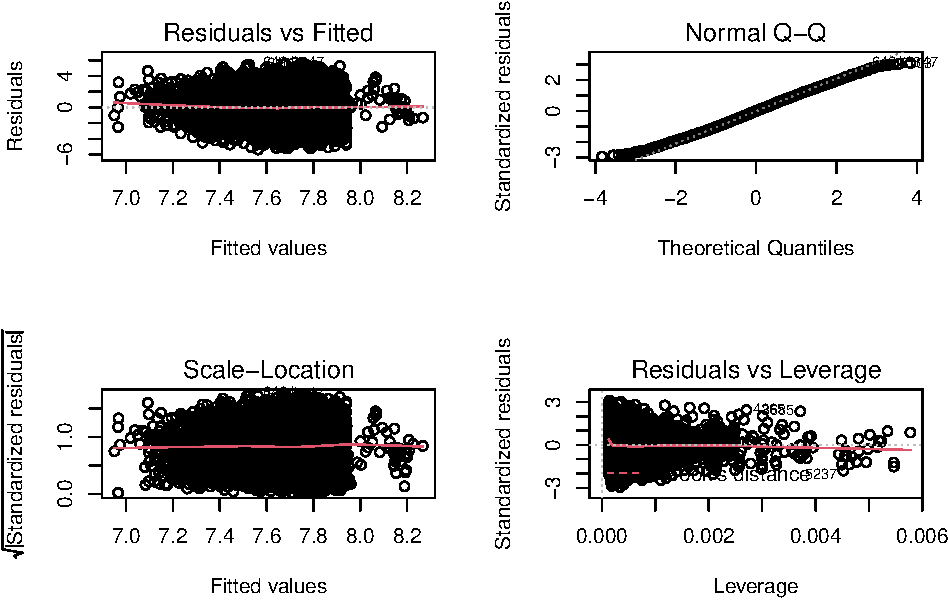
\includegraphics{HW-11-05_files/figure-latex/unnamed-chunk-4-1.pdf}

\begin{Shaded}
\begin{Highlighting}[]
\NormalTok{car}\SpecialCharTok{::}\FunctionTok{scatterplotMatrix}\NormalTok{(df[, }\FunctionTok{c}\NormalTok{(}\StringTok{\textquotesingle{}rate\textquotesingle{}}\NormalTok{, }\StringTok{\textquotesingle{}views\textquotesingle{}}\NormalTok{, }\StringTok{\textquotesingle{}length\textquotesingle{}}\NormalTok{, }\StringTok{\textquotesingle{}ratings\textquotesingle{}}\NormalTok{)])}
\end{Highlighting}
\end{Shaded}

\includegraphics{HW-11-05_files/figure-latex/unnamed-chunk-4-2.pdf}

\begin{Shaded}
\begin{Highlighting}[]
\NormalTok{k6 }\OtherTok{\textless{}{-}} \FunctionTok{lm}\NormalTok{(df}\SpecialCharTok{$}\NormalTok{ratings }\SpecialCharTok{\textasciitilde{}}\NormalTok{ df}\SpecialCharTok{$}\NormalTok{length)}
\FunctionTok{summary}\NormalTok{(k6)}
\end{Highlighting}
\end{Shaded}

\begin{verbatim}
## 
## Call:
## lm(formula = df$ratings ~ df$length)
## 
## Residuals:
##    Min     1Q Median     3Q    Max 
## -150.0  -17.8  -14.3   -5.2 3783.7 
## 
## Coefficients:
##             Estimate Std. Error t value Pr(>|t|)    
## (Intercept) 14.68067    1.05106  13.967   <2e-16 ***
## df$length    0.02633    0.00319   8.254   <2e-16 ***
## ---
## Signif. codes:  0 '***' 0.001 '**' 0.01 '*' 0.05 '.' 0.1 ' ' 1
## 
## Residual standard error: 74.67 on 9607 degrees of freedom
## Multiple R-squared:  0.007041,   Adjusted R-squared:  0.006938 
## F-statistic: 68.12 on 1 and 9607 DF,  p-value: < 2.2e-16
\end{verbatim}

\begin{Shaded}
\begin{Highlighting}[]
\FunctionTok{sprintf}\NormalTok{(}\StringTok{"a1 is \%d"}\NormalTok{, (a1    }\OtherTok{\textless{}{-}} \FunctionTok{sign}\NormalTok{(}\FunctionTok{cor}\NormalTok{(df}\SpecialCharTok{$}\NormalTok{views,df}\SpecialCharTok{$}\NormalTok{ratings))))}
\end{Highlighting}
\end{Shaded}

\begin{verbatim}
## [1] "a1 is 1"
\end{verbatim}

\begin{Shaded}
\begin{Highlighting}[]
\FunctionTok{sprintf}\NormalTok{(}\StringTok{"a2 is \%d"}\NormalTok{, (a2    }\OtherTok{\textless{}{-}} \FunctionTok{sign}\NormalTok{(}\FunctionTok{cor}\NormalTok{(df}\SpecialCharTok{$}\NormalTok{rating, df}\SpecialCharTok{$}\NormalTok{length))))}
\end{Highlighting}
\end{Shaded}

\begin{verbatim}
## [1] "a2 is 1"
\end{verbatim}

\begin{Shaded}
\begin{Highlighting}[]
\FunctionTok{sprintf}\NormalTok{(}\StringTok{"a3 is \%d"}\NormalTok{, (a3    }\OtherTok{\textless{}{-}} \FunctionTok{sign}\NormalTok{(}\FunctionTok{cor}\NormalTok{(df}\SpecialCharTok{$}\NormalTok{ratings, df}\SpecialCharTok{$}\NormalTok{rate))))}
\end{Highlighting}
\end{Shaded}

\begin{verbatim}
## [1] "a3 is 1"
\end{verbatim}

\begin{Shaded}
\begin{Highlighting}[]
\FunctionTok{sprintf}\NormalTok{(}\StringTok{"adir(estimate) is \%d"}\NormalTok{,(adir }\OtherTok{\textless{}{-}}\NormalTok{ a1}\SpecialCharTok{*}\NormalTok{a2}\SpecialCharTok{*}\NormalTok{a3))}
\end{Highlighting}
\end{Shaded}

\begin{verbatim}
## [1] "adir(estimate) is 1"
\end{verbatim}

\begin{Shaded}
\begin{Highlighting}[]
\CommentTok{\#stargazer(mod1, mod2, type = "text")}
\end{Highlighting}
\end{Shaded}

\begin{Shaded}
\begin{Highlighting}[]
\DocumentationTok{\#\# corrplot takes a correlation matrix as an arument}
  \CommentTok{\# needs the corrplot package}
\NormalTok{corrplot}\SpecialCharTok{::}\FunctionTok{corrplot}\NormalTok{(}\FunctionTok{cor}\NormalTok{(df),}\AttributeTok{method =} \StringTok{"color"}\NormalTok{,}\AttributeTok{order=}\StringTok{"AOE"}\NormalTok{, }
                   \AttributeTok{diag=}\ConstantTok{FALSE}\NormalTok{, }\AttributeTok{addCoef.col =} \StringTok{"black"}\NormalTok{, }\AttributeTok{addCoefasPercent =} \ConstantTok{TRUE}\NormalTok{)}
\end{Highlighting}
\end{Shaded}

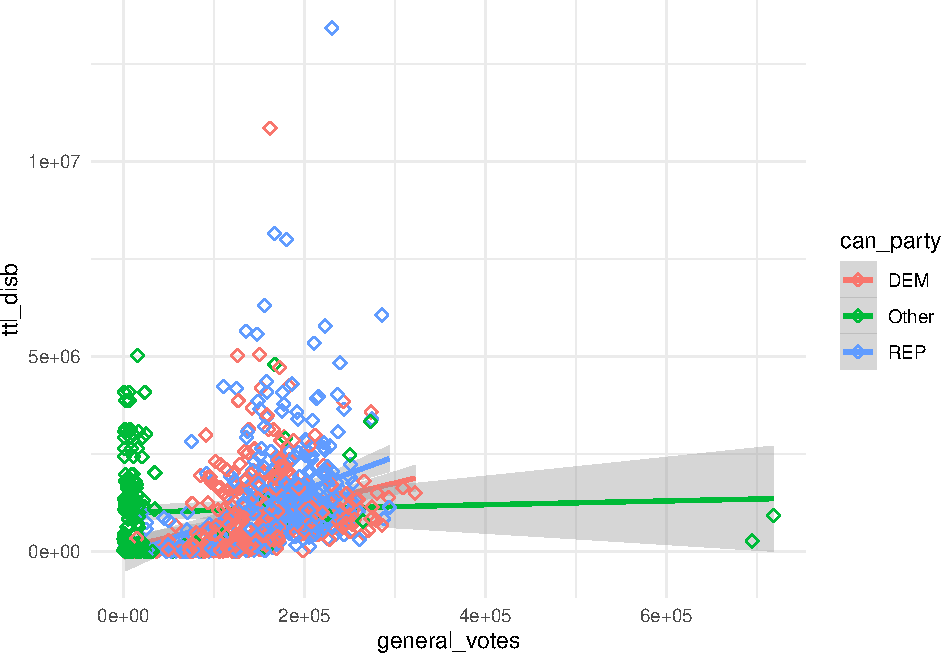
\includegraphics{HW-11-05_files/figure-latex/unnamed-chunk-7-1.pdf}

\begin{Shaded}
\begin{Highlighting}[]
\FunctionTok{cor}\NormalTok{(df}\SpecialCharTok{$}\NormalTok{ratings, df}\SpecialCharTok{$}\NormalTok{rate)}
\end{Highlighting}
\end{Shaded}

\begin{verbatim}
## [1] 0.1279075
\end{verbatim}

\begin{Shaded}
\begin{Highlighting}[]
\FunctionTok{cor}\NormalTok{(df}\SpecialCharTok{$}\NormalTok{views, df}\SpecialCharTok{$}\NormalTok{ratings)}
\end{Highlighting}
\end{Shaded}

\begin{verbatim}
## [1] 0.7189812
\end{verbatim}

\begin{Shaded}
\begin{Highlighting}[]
\FunctionTok{cor}\NormalTok{(df}\SpecialCharTok{$}\NormalTok{views, df}\SpecialCharTok{$}\NormalTok{rate)}
\end{Highlighting}
\end{Shaded}

\begin{verbatim}
## [1] 0.1042721
\end{verbatim}

\begin{Shaded}
\begin{Highlighting}[]
\FunctionTok{cor}\NormalTok{(df}\SpecialCharTok{$}\NormalTok{views, df}\SpecialCharTok{$}\NormalTok{length)}
\end{Highlighting}
\end{Shaded}

\begin{verbatim}
## [1] 0.03512544
\end{verbatim}

\begin{Shaded}
\begin{Highlighting}[]
\FunctionTok{cor}\NormalTok{(df}\SpecialCharTok{$}\NormalTok{ratings, df}\SpecialCharTok{$}\NormalTok{length)}
\end{Highlighting}
\end{Shaded}

\begin{verbatim}
## [1] 0.08391187
\end{verbatim}

\begin{Shaded}
\begin{Highlighting}[]
\FunctionTok{cor}\NormalTok{(df}\SpecialCharTok{$}\NormalTok{rate, df}\SpecialCharTok{$}\NormalTok{length)}
\end{Highlighting}
\end{Shaded}

\begin{verbatim}
## [1] 0.1568035
\end{verbatim}

Discuss of Omitted Variables

\begin{enumerate}
\def\labelenumi{\alph{enumi}.}
\setcounter{enumi}{1}
\tightlist
\item
  Provide a story for why there might be a reverse causal pathway (from
  the number of views to the average rating). Argue whether the
  direction of bias is towards zero or away from zero.
\end{enumerate}

\begin{Shaded}
\begin{Highlighting}[]
\NormalTok{c3 }\OtherTok{\textless{}{-}} \FunctionTok{lm}\NormalTok{(df}\SpecialCharTok{$}\NormalTok{ratings }\SpecialCharTok{\textasciitilde{}}\NormalTok{ df}\SpecialCharTok{$}\NormalTok{views)}
\FunctionTok{summary}\NormalTok{(c3)}
\end{Highlighting}
\end{Shaded}

\begin{verbatim}
## 
## Call:
## lm(formula = df$ratings ~ df$views)
## 
## Residuals:
##      Min       1Q   Median       3Q      Max 
## -1472.88    -7.44    -5.76    -0.73  1408.03 
## 
## Coefficients:
##              Estimate Std. Error t value Pr(>|t|)    
## (Intercept) 7.1103069  0.5478719   12.98   <2e-16 ***
## df$views    0.0014495  0.0000143  101.39   <2e-16 ***
## ---
## Signif. codes:  0 '***' 0.001 '**' 0.01 '*' 0.05 '.' 0.1 ' ' 1
## 
## Residual standard error: 52.08 on 9607 degrees of freedom
## Multiple R-squared:  0.5169, Adjusted R-squared:  0.5169 
## F-statistic: 1.028e+04 on 1 and 9607 DF,  p-value: < 2.2e-16
\end{verbatim}

\begin{Shaded}
\begin{Highlighting}[]
\FunctionTok{stargazer}\NormalTok{(c3, }\AttributeTok{type =} \StringTok{\textquotesingle{}text\textquotesingle{}}\NormalTok{ )}
\end{Highlighting}
\end{Shaded}

\begin{verbatim}
## 
## ================================================
##                         Dependent variable:     
##                     ----------------------------
##                               ratings           
## ------------------------------------------------
## views                         0.001***          
##                              (0.00001)          
##                                                 
## Constant                      7.110***          
##                               (0.548)           
##                                                 
## ------------------------------------------------
## Observations                   9,609            
## R2                             0.517            
## Adjusted R2                    0.517            
## Residual Std. Error      52.084 (df = 9607)     
## F Statistic         10,280.550*** (df = 1; 9607)
## ================================================
## Note:                *p<0.1; **p<0.05; ***p<0.01
\end{verbatim}

\begin{Shaded}
\begin{Highlighting}[]
\FunctionTok{sprintf}\NormalTok{(}\StringTok{"a1 is \%d"}\NormalTok{, (a1 }\OtherTok{\textless{}{-}} \FunctionTok{sign}\NormalTok{(}\FunctionTok{cor}\NormalTok{(df}\SpecialCharTok{$}\NormalTok{views,df}\SpecialCharTok{$}\NormalTok{rate))))}
\end{Highlighting}
\end{Shaded}

\begin{verbatim}
## [1] "a1 is 1"
\end{verbatim}

\begin{enumerate}
\def\labelenumi{\alph{enumi}.}
\setcounter{enumi}{2}
\tightlist
\item
  You are considering adding a new variable, \texttt{rating}, which
  represents the total number of ratings. Explain how this would affect
  your measurement goal.
\end{enumerate}

\begin{Shaded}
\begin{Highlighting}[]
\NormalTok{c9 }\OtherTok{\textless{}{-}}\FunctionTok{lm}\NormalTok{(df}\SpecialCharTok{$}\NormalTok{views }\SpecialCharTok{\textasciitilde{}}\NormalTok{ df}\SpecialCharTok{$}\NormalTok{rate }\SpecialCharTok{+}\NormalTok{ df}\SpecialCharTok{$}\NormalTok{length)}
\NormalTok{c10 }\OtherTok{\textless{}{-}}\FunctionTok{lm}\NormalTok{(df}\SpecialCharTok{$}\NormalTok{views }\SpecialCharTok{\textasciitilde{}}\NormalTok{ df}\SpecialCharTok{$}\NormalTok{rate }\SpecialCharTok{+}\NormalTok{ df}\SpecialCharTok{$}\NormalTok{length }\SpecialCharTok{+}\NormalTok{ df}\SpecialCharTok{$}\NormalTok{ratings)}

\CommentTok{\#summary(c9, c10)}
\FunctionTok{anova}\NormalTok{(c9)}
\end{Highlighting}
\end{Shaded}

\begin{verbatim}
## Analysis of Variance Table
## 
## Response: df$views
##             Df     Sum Sq    Mean Sq F value  Pr(>F)    
## df$rate      1 1.4431e+11 1.4431e+11 105.629 < 2e-16 ***
## df$length    1 4.7968e+09 4.7968e+09   3.511 0.06099 .  
## Residuals 9606 1.3124e+13 1.3662e+09                    
## ---
## Signif. codes:  0 '***' 0.001 '**' 0.01 '*' 0.05 '.' 0.1 ' ' 1
\end{verbatim}

\begin{Shaded}
\begin{Highlighting}[]
\FunctionTok{anova}\NormalTok{(c10)}
\end{Highlighting}
\end{Shaded}

\begin{verbatim}
## Analysis of Variance Table
## 
## Response: df$views
##              Df     Sum Sq    Mean Sq    F value    Pr(>F)    
## df$rate       1 1.4431e+11 1.4431e+11   216.5921 < 2.2e-16 ***
## df$length     1 4.7968e+09 4.7968e+09     7.1993  0.007306 ** 
## df$ratings    1 6.7242e+12 6.7242e+12 10091.9994 < 2.2e-16 ***
## Residuals  9605 6.3997e+12 6.6629e+08                         
## ---
## Signif. codes:  0 '***' 0.001 '**' 0.01 '*' 0.05 '.' 0.1 ' ' 1
\end{verbatim}

\begin{Shaded}
\begin{Highlighting}[]
\FunctionTok{anova}\NormalTok{(c9, c10)}
\end{Highlighting}
\end{Shaded}

\begin{verbatim}
## Analysis of Variance Table
## 
## Model 1: df$views ~ df$rate + df$length
## Model 2: df$views ~ df$rate + df$length + df$ratings
##   Res.Df        RSS Df  Sum of Sq     F    Pr(>F)    
## 1   9606 1.3124e+13                                  
## 2   9605 6.3997e+12  1 6.7242e+12 10092 < 2.2e-16 ***
## ---
## Signif. codes:  0 '***' 0.001 '**' 0.01 '*' 0.05 '.' 0.1 ' ' 1
\end{verbatim}

When you use anova(lm.1,lm.2,test=``Chisq''), it performs the Chi-square
test to compare lm.1 and lm.2 (i.e.~it tests whether reduction in the
residual sum of squares are statistically significant or not). Note that
this makes sense only if lm.1 and lm.2 are nested models.

For example, in the 1st anova that you used, the p-value of the test is
0.82. It means that the fitted model ``modelAdd'' is not significantly
different from modelGen at the level of α=0.05 . However, using the
p-value in the 3rd anova, the model ``modelRec'' is significantly
different form model ``modelGen'' at α=0.1.

\end{document}
